\documentclass{article}

%%% Fill details here (in the second brackets)
\newcommand{\name}{Sam Teeter}     % Your name (First Last)
\newcommand{\wustlkey}{teeters}             % Your WUSTL Key
%%%



%%%%%%%%%%%%%%%%%%%%%% Formatting Stuff %%%%%%%%%%%%%%%%%%%%%%%%%%%
\usepackage{times}
\usepackage[T1]{fontenc}

\setlength{\parskip}{1em}\setlength{\parindent}{0pt}
\linespread{1.25}
\usepackage[margin=0.7in,top=1in]{geometry}\usepackage{fancyhdr}
\pagestyle{fancy}\lhead{\bf \name}\rhead{\bf \wustlkey}\cfoot{\thepage}
\newcommand{\info}{\clearpage \subsection*{Information}}
\newcommand{\solution}[1]{\clearpage \subsection*{Solution #1}}
\newcommand{\spart}[1]{\paragraph{(#1)}}
%%%%%%%%%%%%%%%%%%%%%%%%%%%%%%%%%%%%%%%%%%%%%%%%%%%%%%%%%%%%%%%%%%%


%%% Add any more packages if you want to
\usepackage{amsmath,graphicx}
\usepackage{multirow}


\begin{document}
%%%%% Main Body goes here

% Begin solution to every problem like this.
\solution{1}

\spart{a} Outputs for the \texttt{get\_centers} function:

\begin{figure*}[!h]
  \centering
  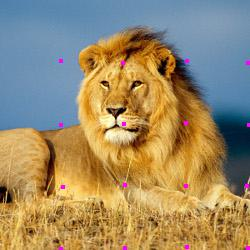
\includegraphics[height=10em]{./code/outputs/prob1a_25_centers.jpg}
  \caption{K=25}
\end{figure*}

\begin{figure*}[!h]
  \centering
  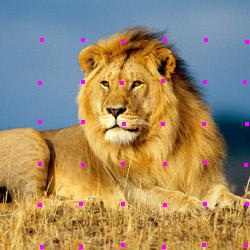
\includegraphics[height=10em]{./code/outputs/prob1a_49_centers.jpg}
  \caption{K=49}
\end{figure*}

\begin{figure*}[!h]
  \centering
  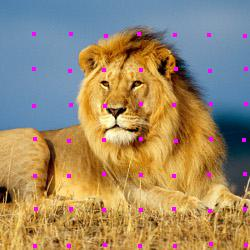
\includegraphics[height=10em]{./code/outputs/prob1a_64_centers.jpg}
  \caption{K=64}
\end{figure*}

\begin{figure*}[!h]
  \centering
  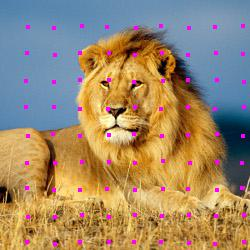
\includegraphics[height=10em]{./code/outputs/prob1a_100_centers.jpg}
  \caption{K=100}
\end{figure*}


\spart{b} Here are the outputs from my \texttt{slic} function. After experimenting, I set the spatial weight value to 5 (leaving the intensity weight at 1). I evaluated images based on the criteria that superpixels should be a) more or less spatially contiguous, and b) capture visually informative regions of the image. I found that a value of 4 or 5 gave the best results for this image. (I also tried normalizing the spatial and intensity distances to a common scale, but I found that this did not improve results).

\begin{figure*}[!h]
	\centering
	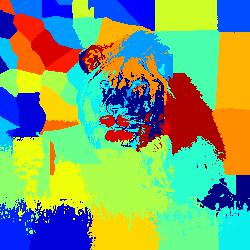
\includegraphics[height=10em]{code/outputs/prob1b_25.jpg}
	\caption{K=25}
\end{figure*}

\begin{figure*}[!h]
	\centering
	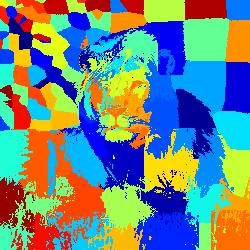
\includegraphics[height=10em]{code/outputs/prob1b_49.jpg}
	\caption{K=49}
\end{figure*}

\begin{figure*}[!h]
	\centering
	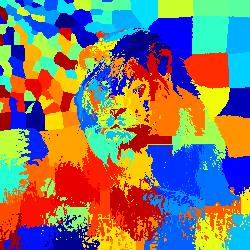
\includegraphics[height=10em]{code/outputs/prob1b_64.jpg}
	\caption{K=64}
\end{figure*}

\begin{figure*}[!h]
	\centering
	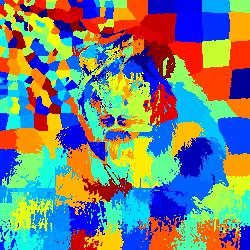
\includegraphics[height=10em]{code/outputs/prob1b_100.jpg}
	\caption{K=100}
\end{figure*}

\solution{2}

\spart{a} Experimental results after 50 epochs:

\begin{center}
\begin{tabular}{ c c c c c c c }
\hline
\multirow{2}{*}{Batch size} & 
\multirow{2}{*}{Learning rate} & 
\multirow{2}{*}{Hidden units} & 
\multicolumn{2}{c}{ Training } &
\multicolumn{2}{c}{ Validation } \\
	&&& Soft-max loss & Accuracy & Soft-max loss & Accuracy \\
\hline
50 & \textbf{.001} & 1024 & .5390 & 85.70\% & .4732 & 88.80\% \\
50 & \textbf{.005} & 1024 & .5623 & 83.12\% & .4915 & 85.10\% \\
50 & \textbf{.010} & 1024 & .8127 & 72.78\% & .7115 & 75.7\% \\
\textbf{10} & .001 & 1024 & .5287 & 83.40\% & .4916 & 85.2\% \\
\textbf{25} & .001 & 1024 & .4582 & 86.52\% & .4069 & 89.40\% \\
\textbf{100} & .001 & 1024 & .7639 & 80.45\% & .6991 & 83.90\% \\
50 & .001 & \textbf{128} & .4844 & 87.26\% & .4394 & 89.6\% \\
50 & .001 & \textbf{256} & .5067 & 87.72\% & .4498 & 90.40\% \\
50 & .001 & \textbf{512} & .5119 & 86.78\% & .4619 & 89.30\% \\
50 & .001 & \textbf{2048} & .6143 & 81.90\% & .5632 & 84.70\% \\
25 & .001 & 256 & .4566 & 87.24\% & .3818 & 90.60\% \\
\hline
\end{tabular}
\end{center}

The final trial combines the optimal values of each variable in the previous trials. Note that the accuracy statistics are only slightly improved from the (hidden units = 256) trial, suggesting that the number of hidden units may be the dominant variable. 

Xavier initialization chooses the initial weights from a distribution with mean 0 and variance equal to $\frac{1}{n_\text{in}}$ where $n_\text{in}$ is the number of inputs to the neuron. In brief, this is because we want the variance of input and output to be the same, so that the variance of the signal does not diminish (or increase) as it penetrates deeper into the network. It can be shown that the variance of the output is proportional to $n$ x the variance of the weights themselves, so setting the input distribution's variance to $\frac{1}{n}$ accomplishes this.

\spart{b} Results with momentum:

\begin{center}
\begin{tabular}{ c c c c c c c }
\hline
\multirow{2}{*}{Batch size} & 
\multirow{2}{*}{Learning rate} & 
\multirow{2}{*}{Hidden units} & 
\multicolumn{2}{c}{ Training } &
\multicolumn{2}{c}{ Validation } \\
	&&& Soft-max loss & Accuracy & Soft-max loss & Accuracy \\
\hline
25 & .001 & 1024 & .005347 & 98.8\% & .1027 & 97.2\% \\
50 & .001 & 1024 & .01153 & 96.96\% & .1392 & 96.1\% \\
100 & .001 & 1024 & .01929 & 94.5\% & .1925 & 95.1\% \\
25 & .001 & 128 & .006691 & 98.12\% & .1171 & 96.6\% \\
25 & .001 & 256 & .006241 & 98.4\% & .1007 & 97.2\% \\
25 & .001 & 512 & .006112 & 98.84\% & .1072 & 96.60\% \\
25 & .001 & 2048 & .004417 & 99.00\% & .09782 & 97.00\% \\
25 & .005 & 1024 & .003071 & 100.0\% & .08190 & 97.50\% \\
25 & .010 & 512 & .001047 & 100.0\% & .08555 & 97.70\% \\
\hline
\end{tabular}
\end{center}

Based on these results, momentum greatly increased both the accuracy and the robustness of the gradient descent. It was able to tolerate a much higher learning rate and converged to 100\% accuracy on the training set after only 20 epochs with the right learning parameters. 

\solution{3}

I implemented convolution in the source files as well as convolution + downsampling under the class name \texttt{conv2down}.

\info

This problem set took approximately 16 hours of effort.


I discussed this problem set with:
\begin{itemize}
\item Hao Sun on Piazza
\item Ayan Chakrabarti
\end{itemize}


% Note that you might have to escape some special symbols in URLS like \_
I also got hints from the following sources:
\begin{itemize}
\item Blogger's (very readable!) explanation of Xavier initialization: http://andyljones.tumblr.com/post/110998971763/an-explanation-of-xavier-initialization
\item Article about convolutional layers: http://www.jefkine.com/general/2016/09/05/backpropagation-in-convolutional-neural-networks/
\end{itemize}

\end{document}
\grid
